%-------------------------------------------------------------------------------
\section{Introduction}
%-------------------------------------------------------------------------------
\FloatBarrier\subsection{Ben-Porath model}

The plots below use the parameterization of the Ben-Porath model \citep{Ben-Porath.1967} model parameterized in \citet{Cahuc.2014}.

\begin{figure}[htp]\centering
\caption{Income over the life-cycle}\label{Income over the life-cycle}
\scalebox{0.35}{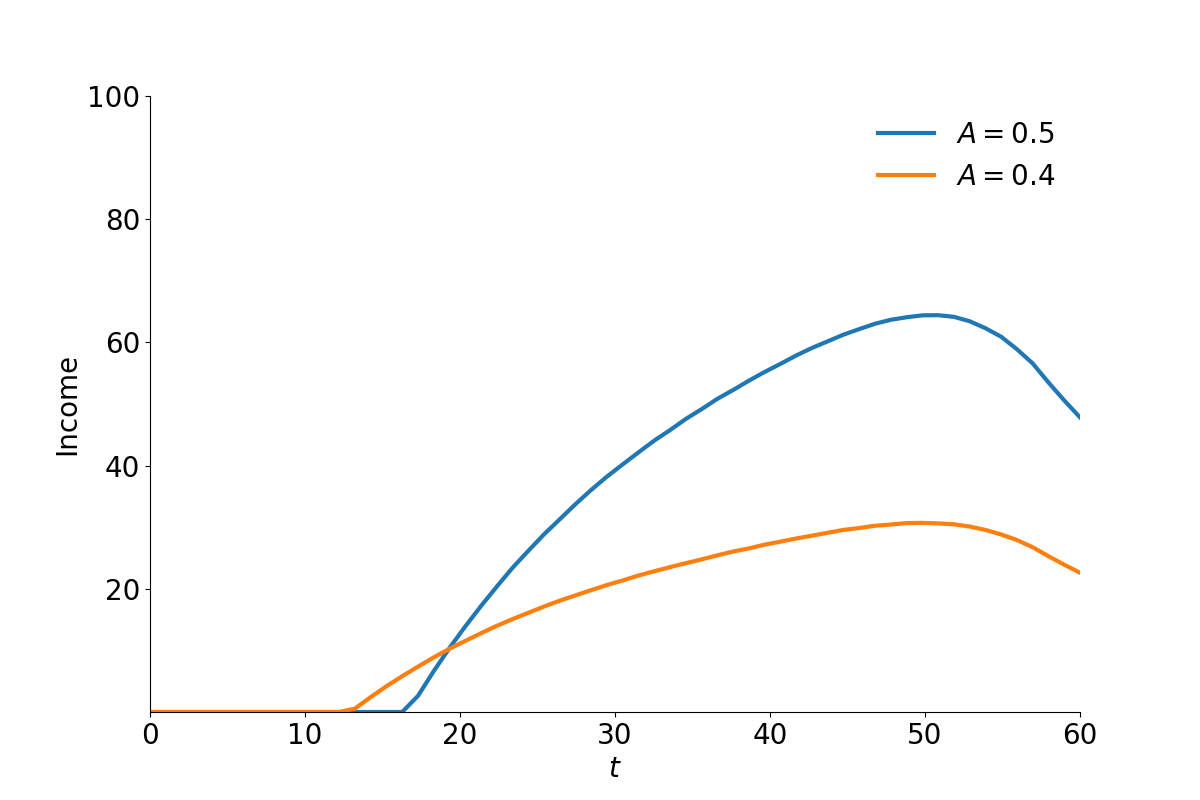
\includegraphics{fig-ben-porath-life-cycle-income}}
\end{figure}

\begin{figure}[htp]\centering
\caption{Stock of human capital over the life-cycle}
\label{Stock of human capital over the life-cycle}
\scalebox{0.35}{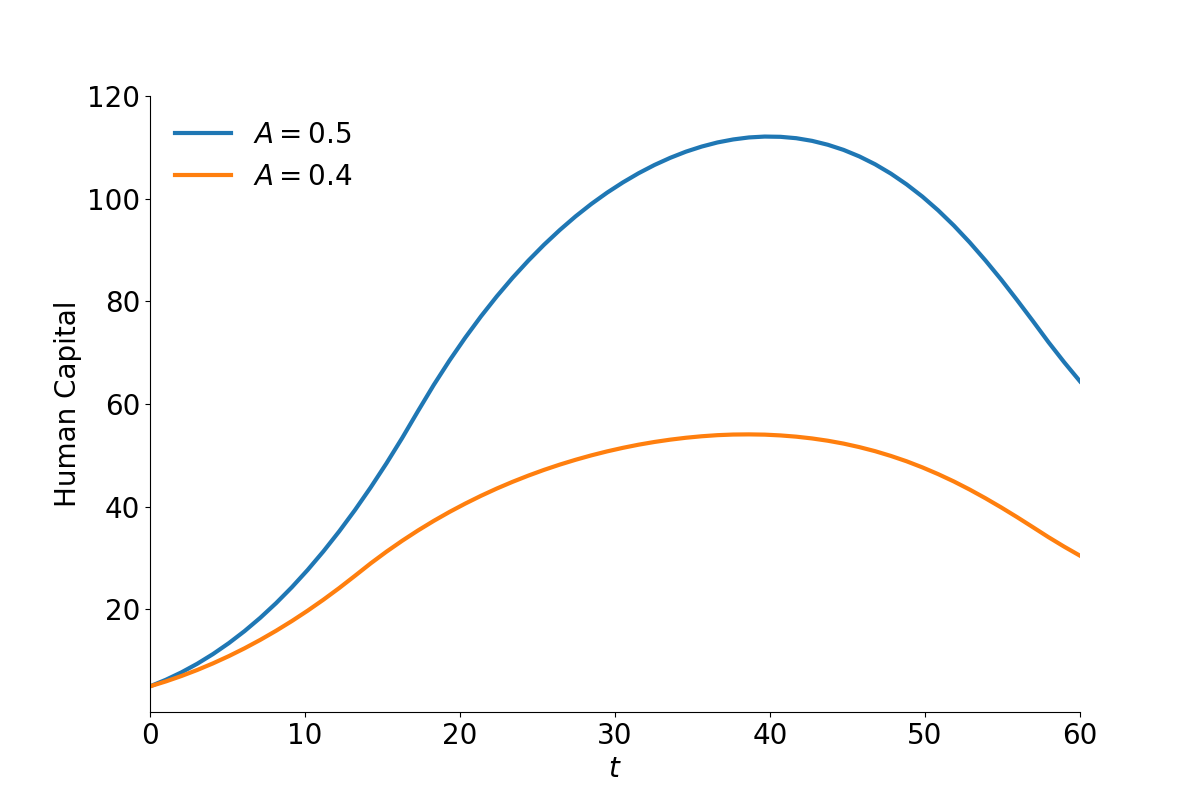
\includegraphics{fig-ben-porath-life-cycle-stock}}
\end{figure}

\begin{figure}[htp]\centering
\caption{Human capital investment over the life-cycle}
\label{Human capital investment over the life-cycle}
\scalebox{0.35}{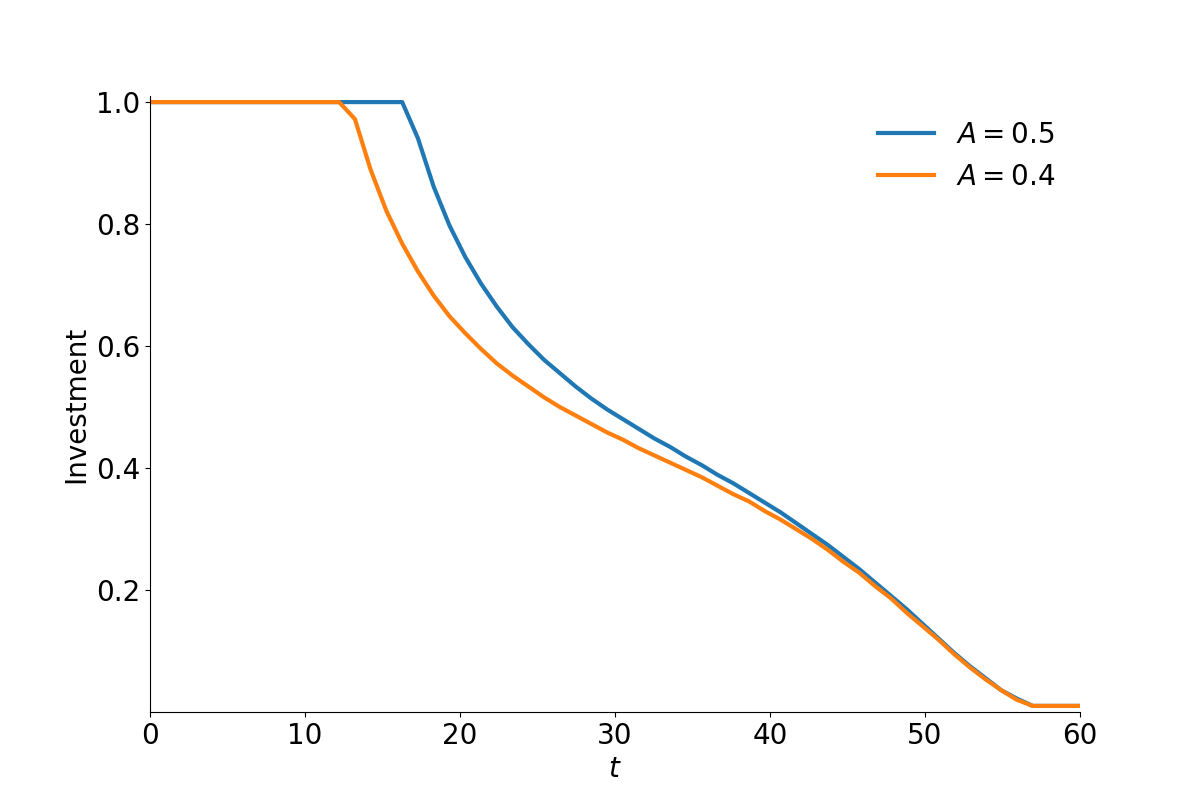
\includegraphics{fig-ben-porath-life-cycle-investment}}
\end{figure}

\begin{figure}[htp]\centering
\caption{Human capital production I}\label{Human capital production I}
\scalebox{0.35}{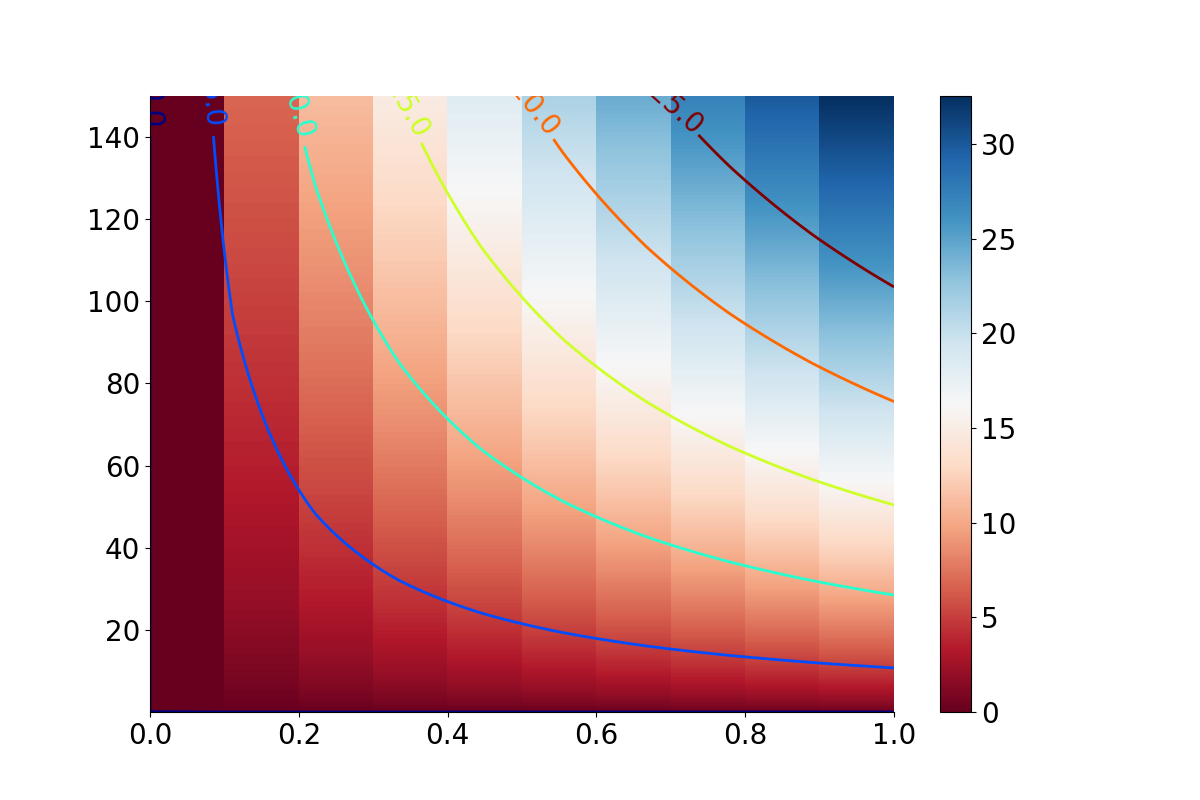
\includegraphics{fig-ben-porath-production-intensity}}
\end{figure}

\begin{figure}[htp]\centering
\caption{Human capital production II}\label{Human capital production II}
\scalebox{0.35}{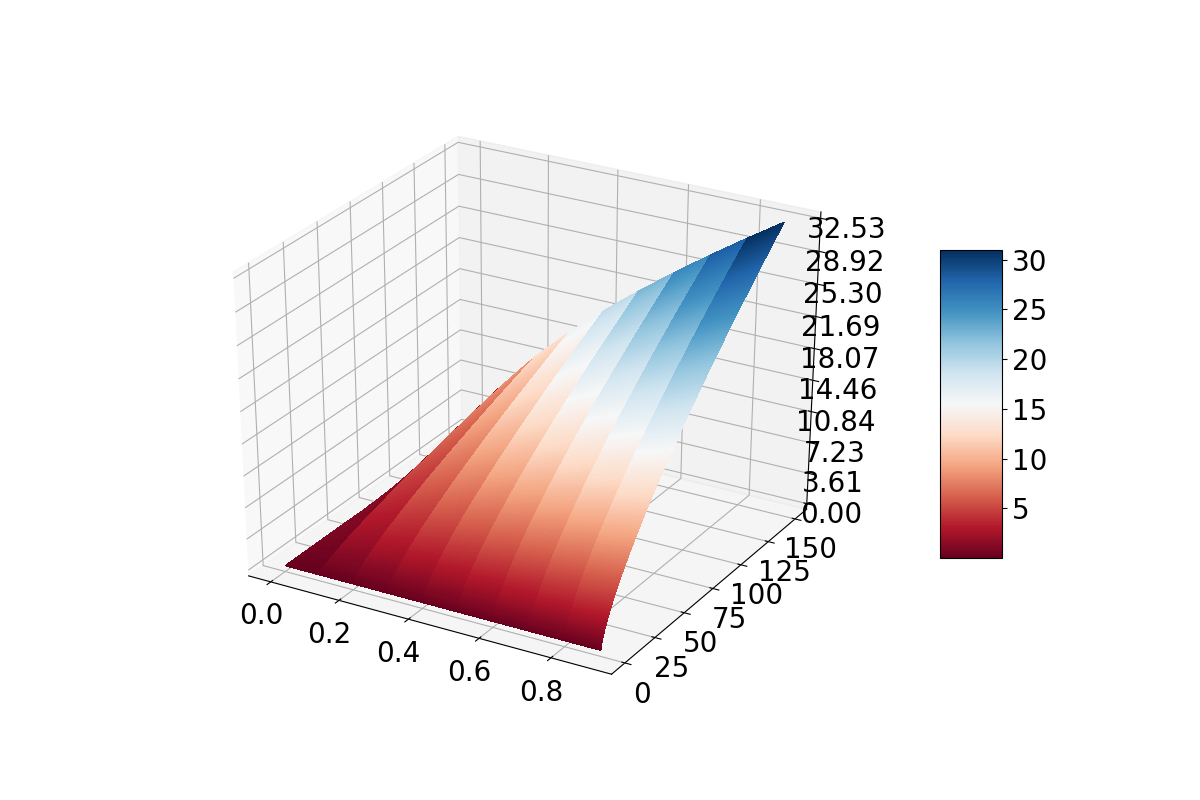
\includegraphics{fig-ben-porath-production-surface}}
\end{figure}

\begin{figure}[htp]\centering
\caption{Income production}\label{Income production}
\scalebox{0.35}{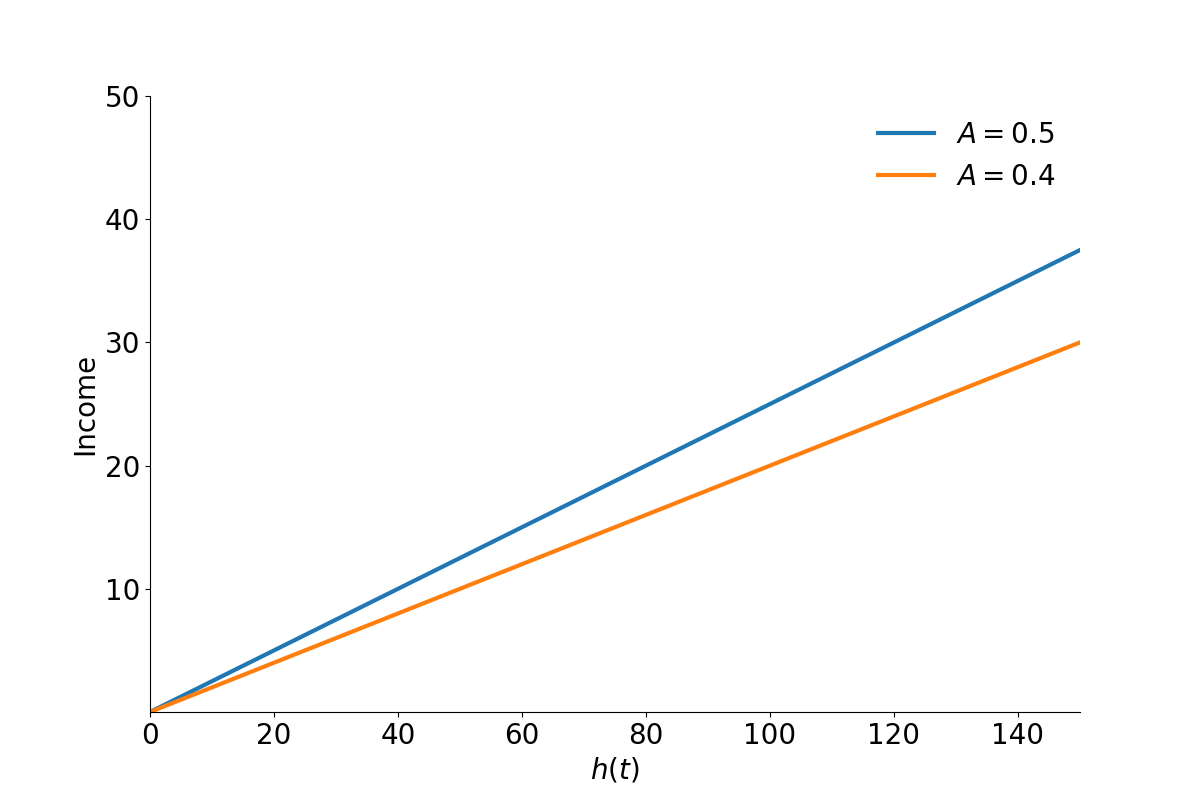
\includegraphics{fig-ben-porath-income}}
\end{figure}
